% !TeX root = ../hw4.tex
\section{Generating a Simple Fractal Tree}

\subsection{Statement}

Generate a fractal tree by repeating a ``fork'' shape with default angle of $45^\circ$.
Scale each repetition of the whole fractal by $\frac{1}{3}$ each iteration.

Experiment with different angles.

\subsection{Method}

\subsubsection{Lindenmayer Systems}
Lindenmayer Systems are commonly referred to as 
\href{https://en.wikipedia.org/wiki/L-system}{L-Systems}. An L-System takes a 
series of production rules and applies them to an 
\href{https://en.wikipedia.org/wiki/Axiom}{axiom}, or initial string for a 
defined number of iterations. To define these L-Systems our approach utilizes a 
\texttt{JSON} file to store the system's variables:

\begin{minted}{json}
{
    "unit": 1,
    "angle": 0.392699082,
    "radius": null,
    "proportion": null,
    "axiom": "G",
    "iterations": 6,
    "randomness": null,
    "rules": {
        "G": "F+[[G]-G]-F[-FG]+G",
        "F": "FF"
    }
}
\end{minted}


\begin{table}
\begin{center}
\begin{tabular}{| c | l |}
    \hline
    \textbf{Name} & \textbf{Description} \\ \hline
    unit & Length of a segment  \\ \hline
    angle & Angle (radians) applied to \verb|+-^v<>|  \\ \hline
    radius & Radius for segments  \\ \hline
    proportion & Changes radius to a proportion of length  \\ \hline
    axiom & Initial string  \\ \hline
    iterations & Number of times to iterate  \\ \hline
    randomness & Perturbation applied to angle  \\ \hline
    rules & Denotes what becomes of characters  \\ \hline
\end{tabular}
\caption{JSON Format of L-System}
\label{table:json_format}
\end{center}
\end{table}

% \todoinline[caption=Define an L-System]{Define an L-System, production rules, and specify the meaning of the different commands.}

\subsubsection{The Lindenmayer System for the Given Problem}
The problem required us to ``shrink'' the original to 1/3 size and apply it to 
each angled protrusion. We accomplished that by coming up with an 
\hyperref[code:prob1_json]{L-System} that grew each previous iteration by a 
factor of 3 each time it went through a new iteration.

\begin{minted}{json}
{
    "unit": 1,
    "angle": 0.785398163,
    "radius": null,
    "proportion": null,
    "axiom": "F",
    "iterations": 7,
    "randomness": null,
    "rules": {
        "F": "GGG[-F][F][+F]",
        "G": "GG"
    }
}
\end{minted}
\label{code:prob1_json}

We were tasked with changing the angle to 90° which resulted in a 
Christmas tree-like structure. We were also tasked with changing the angle to 
120° and it resulted in something similar to a 
\href{https://en.wikipedia.org/wiki/Sierpi%C5%84ski_triangle}{Sierpiński triangle}. 
All three versions are viewable via 
\href{https://sketchfab.com/macattackftw/collections/problem-1}{Sketchfab}. 

\begin{itemize}
    \item \href{https://sketchfab.com/3d-models/prob1-45-a97f7475b6964b9c930796ba985ac255}{45 degrees}
    \item \href{https://sketchfab.com/3d-models/8c7a25615cee4fb4a51ab3deeae154a0}{90 degrees}
    \item \href{https://sketchfab.com/3d-models/b36c6e912ee548b9a549bd8e0bb273c8}{120 degrees}
\end{itemize}

% \todoinline[caption=Give l-system for given problem]{Give the L-System for given problem and discuss how it might be improved or modified.}

\subsubsection{Extending the Lindenmayer Systems to 3D}
The book mentioned symbols to expand the generation into different dimensions. 
We borrowed some of those symbols to generate L-Systems that expanded in the 
$x$, $y$, and $z$ dimensions. We \hyperref[code:prob1_3D_json]{applied} this 
concept to the 45° version of problem 1 and it resulted in a very
\href{https://sketchfab.com/3d-models/prob1-3d-236e501897a945d0a3eb5e4cba37fa3a}{symmetrical tree}.

\begin{figure}
\begin{minted}{json}
{
    "unit": 1,
    "angle": 0.785398163,
    "radius": null,
    "proportion": null,
    "axiom": "F",
    "iterations": 3,
    "randomness": null,
    "rules": {
        "F": "GGG[-F][F][+F][vF][^F][<F][>F]",
        "G": "GG"
    }
}
\end{minted}
\caption*{Problem 1 3D JSON}
\label{code:prob1_3D_json}
\end{figure}

Transitioning to 3D space was incredibly simple due to Blender's mathutils 
Matrix module as seen in the 
\hyperref[code:roll_pitch_yaw]{Roll, Pitch, Yaw Code Block}. We spent a lot of 
time attempting to manipulate Quaternions but found the mathutils module met 
all of our requirements and didn't give us a headache.

\begin{figure}
\begin{minted}{python}
def yaw(self, angle):
    """Yaw the Turtle around its local Z axis."""
    self.mat = matmul(self.mat, Matrix.Rotation(angle, 4, "Z"))

def pitch(self, angle):
    """Pitch the Turtle around its local Y axis."""
    self.mat = matmul(self.mat, Matrix.Rotation(angle, 4, "Y"))

def roll(self, angle):
    """Roll the Turtle around its local X axis."""
    self.mat = matmul(self.mat, Matrix.Rotation(angle, 4, "X"))
\end{minted}
\caption*{Roll, Pitch, Yaw code}
\label{code:roll_pitch_yaw}
\end{figure}

Angle commands such as \texttt{\^} were mapped to pitch function described in 
the \hyperref[code:roll_pitch_yaw]{Roll, Pitch, Yaw Code Block}. So the turtle 
would pitch $\theta$ and if the angle command was \texttt{v} it would pitch 
$-\theta$.


% \todoinline[caption=Defined new 3D commands]{
%     Show how to add more commands to extend the L-Systems into 3D.

%     Mention that we implemented this as the book suggested --- by creating a 3D turtle that can yaw, pitch, and roll.

%     Give minimal examples of each command.
% }

\subsubsection{Further Extensions of the Lindenmayer Systems}
Another concept the book mentioned was moving forward without drawing a line. 
This was accomplished with symbols \texttt{f} and \texttt{g}. Utilizing this 
concept we were able to reproduce the 
\href{https://sketchfab.com/3d-models/cantor-f645d6ae69a748a283a737f44660c5f6}{Cantor Set}.

We were making plant-like structures so we decided that anything over length 1 
would be a ``branch'' and anything else was a ``leaf''. This led to much more 
plant-like visualization of the L-Systems. A good example of this can be seen 
in Figure \ref{fig:a_3d} and Figure \ref{fig:prob1_3d}. We did not have to stop 
at 2 colors. We could have added any number of colors and based it on the 
length or on the iteration. We chose 2 because it demonstrated the concept and 
made the resulting system look better.

\begin{figure}[H]
\centering
\noindent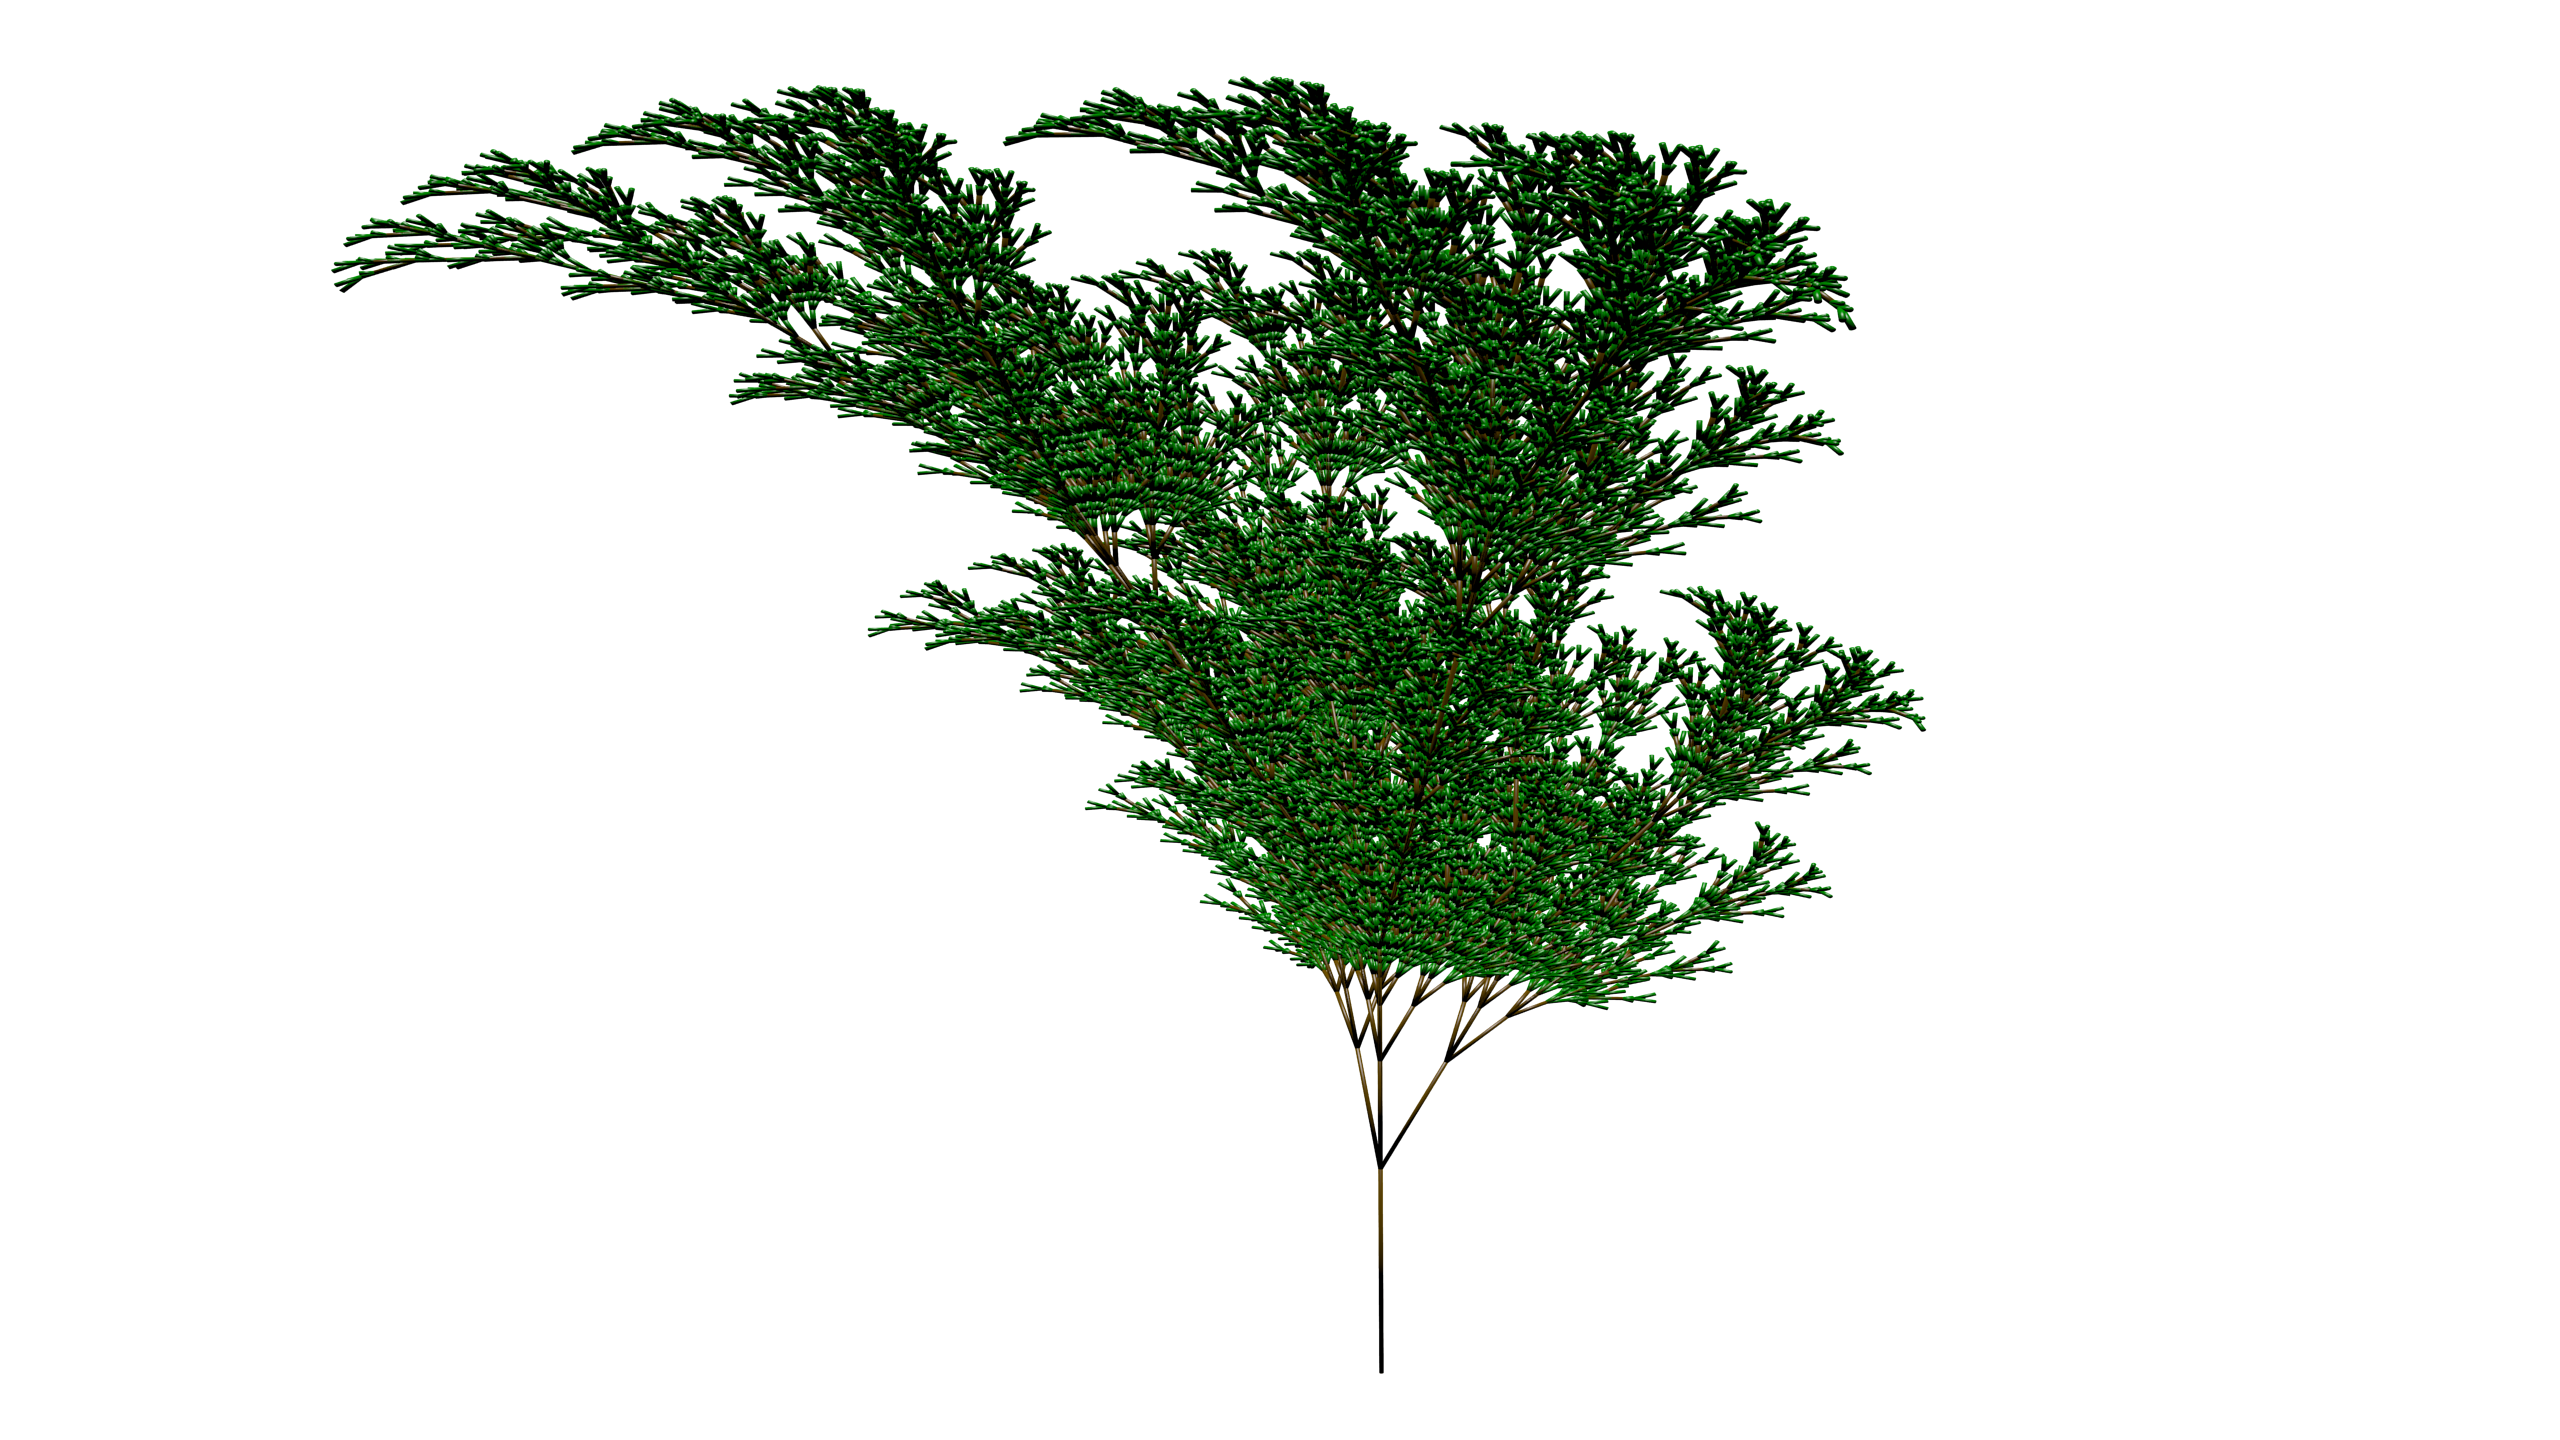
\includegraphics[width=0.75\textwidth]{figures/L-systems/a3d}
\caption[3D L-system Example]{A 3D representation of the book Figure 7.24a}
\label{fig:a_3d}
\end{figure}

\begin{figure}[H]
\centering
\noindent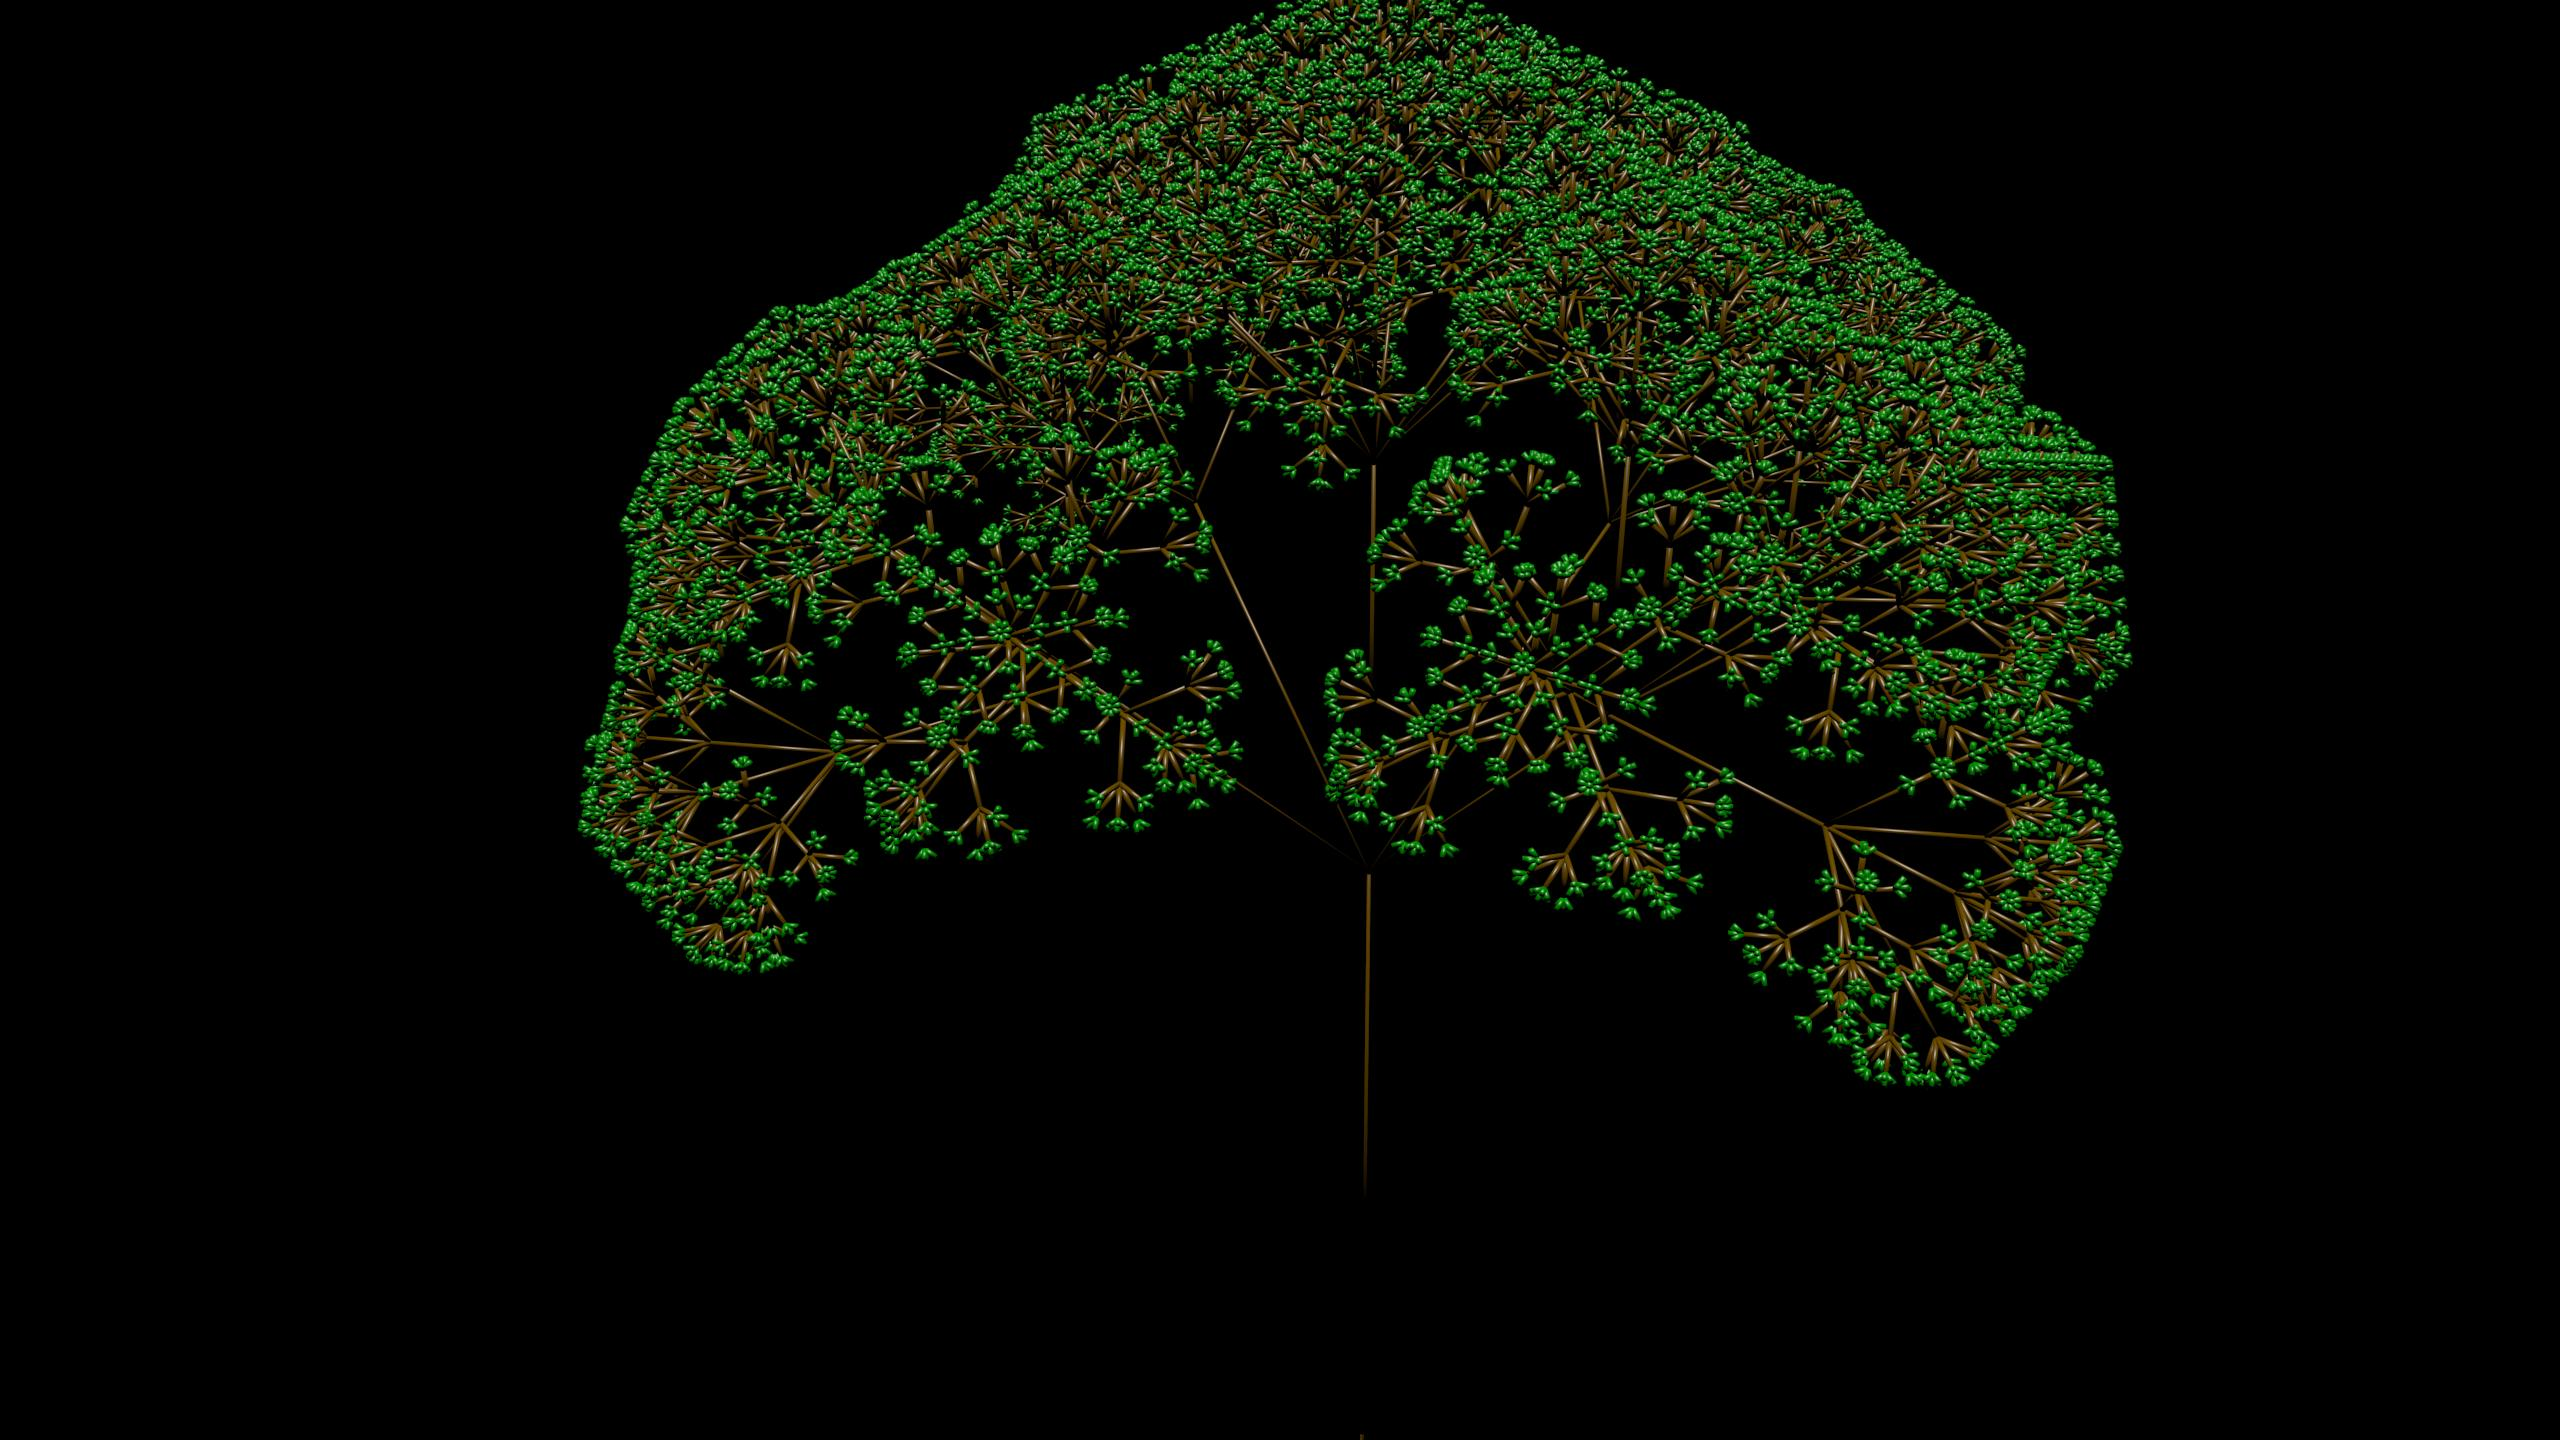
\includegraphics[width=0.75\textwidth]{figures/L-systems/prob13d}
\caption[3D Representation of Problem 1]{A 3D representation of problem 1}
\label{fig:prob1_3d}
\end{figure}

We experimented further with radii proportionality and randomness but the 
results didn't look as good. Radii proportionality did not look good as a 
locked radii and would probably be better if done with a function instead of a 
scaler. Randomness broke the fractal nature of the designs. We found that there 
were many cases where patterns would loop back on themselves and generate 
multiple identical cylinders. Applying the perturbation to angle or length 
resulted in a complete breakdown of the fractal symmetry. It is possible that 
some simple L-System variations may have looked better but we did not find one.

% \todoinline[caption=Further extending the L-System]{Discuss how to add color, radii proportionality, and randomness}
% \todoinline[caption=Add randomness]{
%     Implement randomness.
%     I can think of two ways to do so:
%     First, add an \texttt{r} command that perturbs the immediately following command.
%     This would introduce randomness, but at regular intervals.

%     Second, add a randomness parameter to the constructor, so that if it's set, apply perturbations at random.

%     Mention that adding randomness breaks fractals with backtracking.
% }

\subsection{Implementation}
Implementation of this problem was done in three parts: \texttt{grammar}, 
\texttt{graphics}, and \texttt{turtle}. 

\subsubsection{Grammar}
This section identified which symbols we would utilize as well as how it would 
build the final string. Symbols were defined within a 
\href{https://docs.python.org/3/library/stdtypes.html#frozenset}{frozenset}: 
\mintinline{python}{symbols}. The function: \mintinline{python}{iapply} essentially 
utilizes a generator to apply production rules to the \texttt{axiom} of the 
given iteration.

\subsubsection{Graphics}
Graphics assigns the initial conditions specified in the \texttt{JSON} file. 
The various function mappings are assigned such as:

\begin{minted}{python}
self.mappings = {"F": self.turtle.move, "^": self.turtle.pitch}
\end{minted}

We then iterate through the string (\texttt{commands}), applying the 
appropriate mappings. We keep track of consecutive move commands to determine 
segment length. This serves to reduce the number of cylinders we have to draw 
and it allows us to assign a color scheme based on length.

Cylinders are saved in a dictionary format:
\begin{minted}{python}
cylinders.append(
    {
        "from": start,
        "to": end,
        "radius": self.radius,
        "material": "Branch" if length > 1 else "Leaf",
        "length": length,
    }
)
\end{minted}

\begin{table}
\begin{center}
\begin{tabular}{| c | l |}
    \hline
    \textbf{Name} & \textbf{Description} \\ \hline
    from & Origin \\ \hline
    to & Destination \\ \hline
    radius & Radius for segment \\ \hline
    material & Branch or Leaf dependent on length \\ \hline
    length & Cylinder length  \\ \hline
\end{tabular}
\caption{Dictionary of Cylinders}
\label{table:dict_cylinders}
\end{center}
\end{table}

Table \ref{table:dict_cylinders} defines what each attribute in a cylinder 
means. Due to the quirks of Blender we determined it was better to create a 
single cylinder and then copy it, so for each length we generate a master. The 
master is copied for each cylinder of the same length, while the copy has the 
appropriate \texttt{from - to} applied. This application is done through the 
\mintinline{python}{draw} function. We started to have \texttt{axioms} that 
were hundreds of thousands of characters long. Speed became an issue with 
sufficient iterations so we developed a batch system.  We specify the number of 
jobs we want to run on via command line: 

\texttt{./batch.sh data/b3d.json --jobs 32}

Essentially this chops up the \texttt{cylinders} list into 32 pieces and runs 
them concurrently. Runtimes went from 45 minutes to a few seconds. The 
batch process fires up \texttt{--jobs N} instances of Blender. This can 
quickly consume all RAM. We had to play around with the limits of our 
individual machines to find the maximums. This batch process allowed us to 
break 19,000 cylinders which was a hard threshold we were struggling to surpass. 
We were able to generate 137,000 cylinders without issue utilizing the batch 
method. 

Individually generated \texttt{.blend} files are joined into a 
single entity which reduces the size of the stored 3D object. If the resulting 
\texttt{.fbx} file is under 50MB we were able to upload it to 
\href{https://sketchfab.com/macattackftw/models}{Sketchfab}. 

\subsubsection{Turtle}
The turtle is a very simple python class. Blender's mathutils makes turtles 
very easy to implement. Prior to finding this we spent several days trying to 
get Quaternions working. The \mintinline{python}{turtle} class only has a few 
functions:

\begin{itemize}
    \item push
    \item pop
    \item move
    \item roll
    \item pitch
    \item yaw
    \item position
\end{itemize}

Roll, pitch, and yaw are simply matrix multiplications applied to the existing 
rotation. Move is a matrix multiplication applied to the existing position. 
Push and pop are utilized for setting and then returning to that position 
respectively.

% \todoinline{
%     McGough has seemed to like my (brief) discussion of my previous implementations.
%     We should not give the whole thing, just the interesting bits and pieces.
% }

\subsubsection{Existing Implementations}
\todoinline[caption=Existing impelemtations]{
    Mention all of the existing implementations we found of L-Systems, both 2D and 3D.
    Give links to the easiest to use implementations.

    Show how to use \LaTeX{} to generate them, because he'd like that, and might even find it useful.
}

% \subsubsection{Applying the Production Rules}
% Covered in Graphics subsubsection
% \todoinline[caption=Implementation of the production rules]{Show how to apply the production rules.}

% \subsubsection{A 3D Turtle}
% Covered in the Turtle subsubsection
% \todoinline[caption=Implementation of the 3D turtle]{
%     Show how the 3D turtle was implemented.
%     Be very clear how painful quaternions were and the difficulty of performing the transformations in the local reference frame.

%     Cite the Lindenmaker Blender addon \url{https://github.com/lemurni/lpy-lsystems-blender-addon} and thesis, but mention that the only thing we ripped off was the Turtle.
% }

\subsubsection{Computing the Vertices}
I have no clue what kind of voodoo mathamagic you used to do this.
\todoinline[caption=Implementation of the vertex computation]{
    Discuss the \mintinline{python}{Graphics.compute(lstring)} method and its implementation.
    Be sure to include the data structure it returns and how the material is set.

    Also include the proportional radii, and randomness (once it's implemented).
}

% \subsubsection{Adding Cylinders to the 3D Scene}
% Covered in Graphics subsubsection. I don't think he cares about the details that much in regards to Blender.
% \todoinline[caption=Implementation of adding objects to the scene]{
%     Show how to add a single cylinder to the scene, and mention that it slowed down Blender substantially.

%     Show how to fix this by duplicating cylinders, but mention that there was still a substantial slowdown for large fractals.
% }

% \subsubsection{Parallel Scene Creation}
% He's not going to care about the code to join blender files, though the process is explained above.
% \todoinline[caption=Implementation of batch processing]{
%     Discuss the general idea of the batch mode, but there's no need to give actual code --- other than how to join two files.
% }

\subsubsection{Usage}
We initially designed this to be ran in a single thread with no concurrent 
usage. This proved inadequate for sufficiently large L-Systems. The recommended 
mode of operation is batch and to do so simple generate a \texttt{JSON} file in 
the format shown in the \hyperref[code:prob1_json]{JSON Example}. Save the file 
in whatever folder you wish, then run:

\texttt{./batch.sh data/myJSON.json --jobs N}

To keep things neat we recommend placing the \texttt{JSON} file in the data 
folder. Jobs (\texttt{N}) can be from 1 to as much RAM as your system can 
handle. It is not recommended to go beyond 32 jobs unless you have more than 
16GB of RAM.

The final file will be \texttt{data/myJSON.blend}. All of the 
\texttt{myJSON-job-*-.blend} are from the \texttt{N} jobs scheduled and are the 
individual components of the final \texttt{.blend} file.

% \todoinline[caption=Script usage]{
%     Discuss how to use each of the scripts we created, spending the most time on \texttt{blender.py} and \texttt{batch.sh}.

%     Make sure to point out that the \mintinline{python}{bpy} and \mintinline{python}{mathutils} libraries are provided by Blender, and that to use them we need to run our scripts in funky ways.
% }

\subsection{Results}

\subsubsection{The Lindenmayer System for the Given Problem}
\todoinline[caption=results for given problem]{
    Show our results for the given problem.

    Show the production rules, and generated graphics.
    Play with the scale and the yaw angle.
}

\todoinline[caption=Move experimentation to problem 2]{
    Leave the 3D and other experimentation to problem 2, because it asks you to experiment, and we can get more mileage out of it there.
}

\subsection{Conclusion}
